\documentclass[letterpaper,12pt]{article}
\usepackage{array}
\usepackage{threeparttable}
\usepackage{geometry}
\geometry{letterpaper,tmargin=1in,bmargin=1in,lmargin=1.25in,rmargin=1.25in}
\usepackage{fancyhdr,lastpage}
\pagestyle{fancy}
\lhead{}
\chead{}
\rhead{}
\lfoot{}
\cfoot{}
\rfoot{\footnotesize\textsl{Page \thepage\ of \pageref{LastPage}}}
\renewcommand\headrulewidth{0pt}
\renewcommand\footrulewidth{0pt}
\usepackage[format=hang,font=normalsize,labelfont=bf]{caption}
\usepackage{listings}
\lstset{frame=single,
  language=Python,
  showstringspaces=false,
  columns=flexible,
  basicstyle={\small\ttfamily},
  numbers=none,
  breaklines=true,
  breakatwhitespace=true
  tabsize=3
}
\usepackage{amsmath}
\usepackage{amssymb}
\usepackage{amsthm}
% \usepackage{harvard}
\usepackage{setspace}
\usepackage{float,color}
\usepackage[pdftex]{graphicx}
\usepackage{hyperref}
\hypersetup{colorlinks,linkcolor=red,urlcolor=blue}
\theoremstyle{definition}
\newtheorem{theorem}{Theorem}
\newtheorem{acknowledgement}[theorem]{Acknowledgement}
\newtheorem{algorithm}[theorem]{Algorithm}
\newtheorem{axiom}[theorem]{Axiom}
\newtheorem{case}[theorem]{Case}
\newtheorem{claim}[theorem]{Claim}
\newtheorem{conclusion}[theorem]{Conclusion}
\newtheorem{condition}[theorem]{Condition}
\newtheorem{conjecture}[theorem]{Conjecture}
\newtheorem{corollary}[theorem]{Corollary}
\newtheorem{criterion}[theorem]{Criterion}
\newtheorem{definition}[theorem]{Definition}
\newtheorem{derivation}{Derivation} % Number derivations on their own
\newtheorem{example}[theorem]{Example}
\newtheorem{exercise}[theorem]{Exercise}
\newtheorem{lemma}[theorem]{Lemma}
\newtheorem{notation}[theorem]{Notation}
\newtheorem{problem}[theorem]{Problem}
\newtheorem{proposition}{Proposition} % Number propositions on their own
\newtheorem{remark}[theorem]{Remark}
\newtheorem{solution}[theorem]{Solution}
\newtheorem{summary}[theorem]{Summary}
%\numberwithin{equation}{section}
\bibliographystyle{aer}
\newcommand\ve{\varepsilon}
\newcommand\boldline{\arrayrulewidth{1pt}\hline}


\begin{document}

\begin{flushleft}
  \textbf{\large{Problem Set \#3}} \\
  MACS 30100, Dr. Evans \\
  Julian McClellan
\end{flushleft}

\vspace{5mm}

\noindent\textbf{Problem 1} 
\\
\noindent\textbf{Part (a).} 
\begin{figure}[htb]\centering\captionsetup{width=4.0in}
  \caption{\textbf{Question 1 part(a)}}\label{Figure 1a}
  \fbox{\resizebox{4.0in}{3.0in}{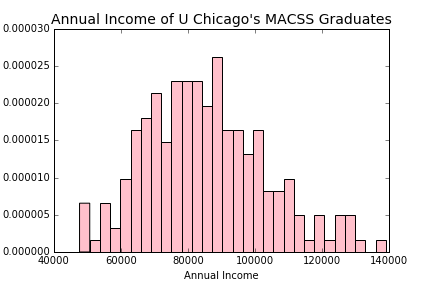
\includegraphics{images/Fig_1a.png}}}
\end{figure}

\\
\noindent\textbf{Part (b).} 
\begin{figure}[H]\centering\captionsetup{width=4.0in}
  \caption{\textbf{Question 1 part(b)}}\label{Figure 1b}
  \fbox{\resizebox{4.0in}{3.0in}{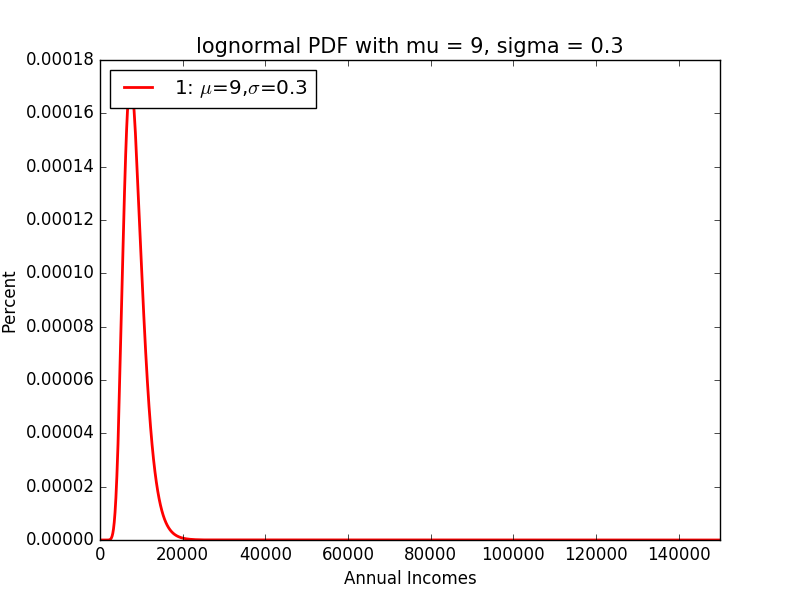
\includegraphics{images/Fig_1b.png}}}
\end{figure}
2 moment (mean and standard deviation) GMM estimated the parameters of a lognormal distribution to be $\mu=11.337\quad and \quad \sigma=0.213$
The value of the criterion function for this parameterization of the distribution
and given this data is $1.735e-13$.

\\
Moments\\
$mean_{data}=85276.824\quad mean_{gmm}=85276.791$
$sd_{data}=17992.542\quad sd_{gmm}=17992.539$

\\
\noindent\textbf{Part (c).}
\begin{figure}[H]\centering\captionsetup{width=4.0in}
  \caption{\textbf{Question 1 part(c)}}\label{Figure 1c}
  \fbox{\resizebox{4.0in}{3.0in}{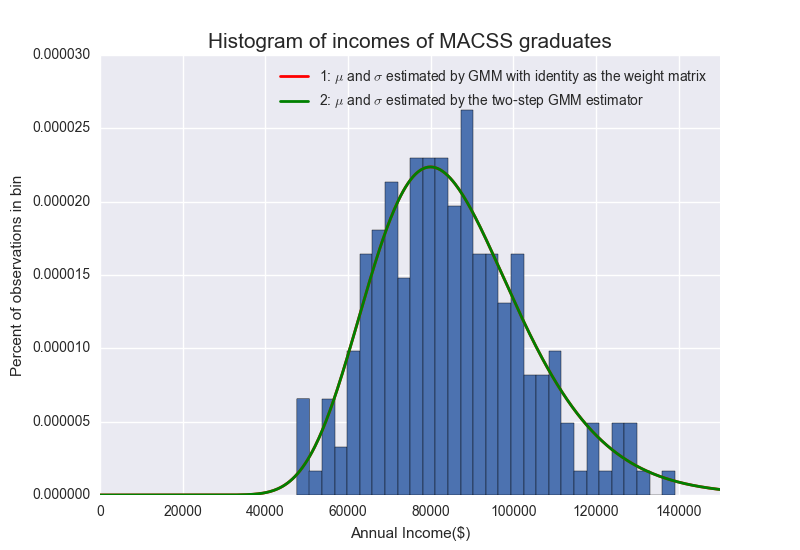
\includegraphics{images/Fig_1c.png}}}
\end{figure}
2 moment (mean and standard deviation) GMM with a 2-step weights matrix estimated the parameters of a lognormal distribution to be $\mu=11.081\quad and \quad \sigma=0.751$
The value of the criterion function for this parameterization of the distribution
and given this data is $-0.0284$.

\\
Moments:\\
\begin{figure}[H]\centering\captionsetup{width=4.0in}
  \caption{\textbf{Question 1 part(d)}}\label{Figure 1d}
  \fbox{\resizebox{4.0in}{3.0in}{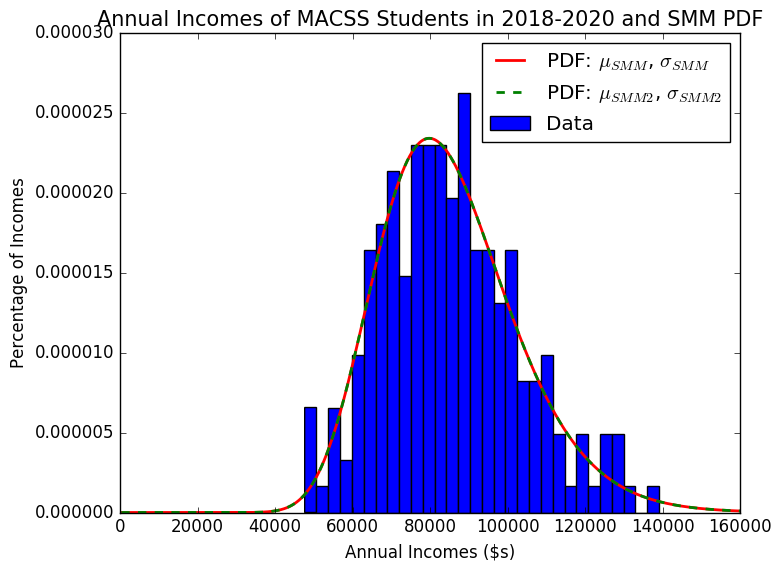
\includegraphics{images/Fig_1d.png}}}
\end{figure}
$mean_{data}=85276.824\quad mean_{gmm}=85276.791$
$sd_{data}=17992.542\quad sd_{gmm}=33028.440$

\\
\noindent\textbf{Part (d).}
3 moment (bins) GMM estimated a the parameters of a lognormal distribution to be $\mu=11.337\quad and \quad \sigma=0.212$

The value of the criterion function for this parameterization of the distribution and given this data is $2.382e-05$

The proportion of incomes in the data between \$0 and \$75,000 = 0.300
The proportion of incomes in the data between \$75,000 and \$100,000 = 0.500
The proportion of incomes in the data between \$100,000 and \$150000 = 0.200
\\
The proportion of incomes in the model between \$0 and \$75,000 = 0.299
The proportion of incomes in the model between \$75,000 and \$100,000 = 0.498
The proportion of incomes in the model between \$100,000 and \$150000 = 0.200


\\
\noindent\textbf{Part (e).}
\begin{figure}[H]\centering\captionsetup{width=4.0in}
  \caption{\textbf{Question 1 part(e)}}\label{Figure 1e}
  \fbox{\resizebox{4.0in}{3.0in}{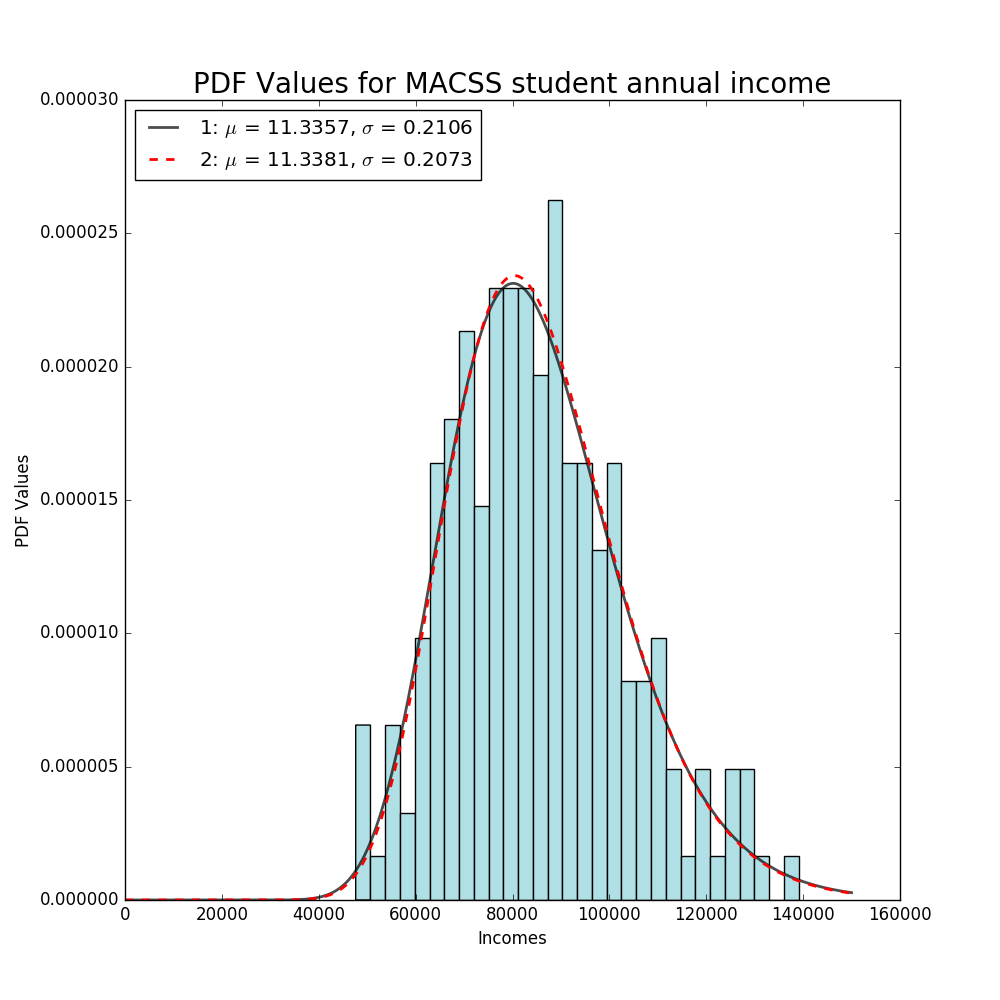
\includegraphics{images/Fig_1e.png}}}
\end{figure}
3 moment (bins) GMM estimated a the parameters of a lognormal distribution to be $\mu=11.336\quad and \quad \sigma=0.197$

The value of the criterion function for this parameterization of the distribution and given this data is $1.125e-13$\\

The proportion of incomes in the data between \$0 and \$75,000 = 0.300\\
The proportion of incomes in the data between \$75,000 and \$100,000 = 0.500\\
The proportion of incomes in the data between \$100,000 and \$150000 = 0.200\\
\\
The proportion of incomes in the model between \$0 and \$75,000 = 0.288\\
The proportion of incomes in the model between \$75,000 and \$100,000 = 0.528\\
The proportion of incomes in the model between \$100,000 and \$150000 = 0.182\\

\\
\\
\noindent\textbf{Part (f).}\\
As one can see, utilizing a two-step weights matrix in part (b) results in a really ill-fitting lognormal pdf. Additionally, using a two-step weights matrix
in part (e) scarcely changes the lognormal pdf from (d) (which itself is quite similar to that in part (b)). \\

Even so, the pdf displayed in red in part (e), the one created using a two-step
weights matrix with the three bin moments, seems to fit my view of the data better. Looking at the above figure, the red pdf has lower values for higher ends of the distribution than the green pdf does. This seems like a more realistic state of affairs for incomes of students just coming out of the master's program. Sure, there will be those able to achieve that level of income, but it seems more realistic to model that fewer will be able to do so.
\\
\noindent\textbf{Problem 2}
\\
\noindent\textbf{Part (a).}
\\
$\beta^{gmm}_{0} = .252\quad \beta^{gmm}_{1} = 0.013\quad\beta^{gmm}_{2} = 0.401\quad \beta^{gmm}_{3} = -0.009992\quad\sigma^{2}_{gmm}=9.11e-06$
The  criterion function value with 2a's GMM estimates = 0.00182
\end{document}
% \noindent\textbf{Part (c).} 
% \begin{figure}[h!]\centering\captionsetup{width=4.0in}
%   \caption{\textbf{1c}}\label{FigExample}
%   \fbox{\resizebox{4.0in}{3.0in}{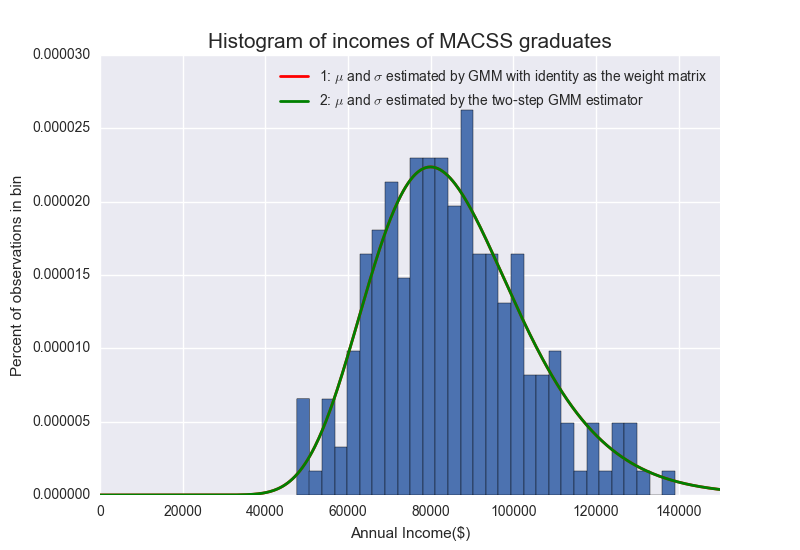
\includegraphics{images/Fig_1c.png}}}
% \end{figure}
% 18.08\% of the time I will be able to pay off the loan in 10 years.

% \noindent\textbf{Part (d).} 
% \begin{figure}[h!]\centering\captionsetup{width=4.0in}
%   \caption{\textbf{1d}}\label{FigExample}
%   \fbox{\resizebox{4.0in}{3.0in}{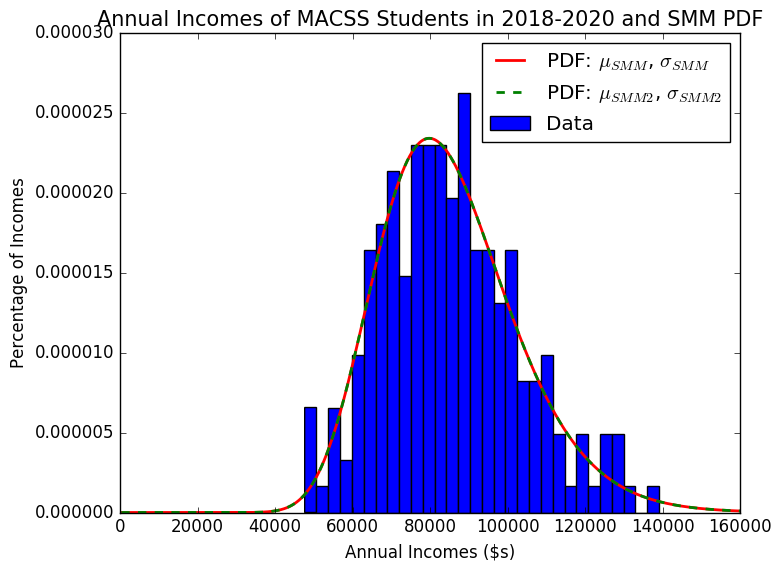
\includegraphics{images/Fig_1d.png}}}
% \end{figure}
% 69.87\% of the time I will be able to pay off the loan in 10 years.
 
% \begin{equation*}
%   \Omega_{j,t} = \left(\frac{\int_{m=4}^\infty(2t + 7m)dm}{\sum_{x=1}^23\sin(\theta_{j,x})}\right) + 7
% \end{equation*}
% You could refer to that object from the equation in math mode $\Omega_{j,t}$ in the sentence. Or if you wanted to talk about the equation, you could remove the asterisks, give it a label, and refer to it with references.
% \begin{equation}\label{EqCoolness}
%   \Omega_{j,t} = \left(\frac{\int_{m=4}^\infty(2t + 7m)dm}{\sum_{x=1}^23\sin(\theta_{j,x})}\right) + 7
% \end{equation}
% Look how cool equation \eqref{EqCoolness} is.

% You might want to include a table in your \LaTeX document. For this, you use the \texttt{tabular} environment.
% \begin{table}[htbp] \centering \captionsetup{width=6.0in}
% \caption{\label{TabExample}\textbf{Sweet example table}}
%   \begin{threeparttable}
%   \begin{tabular}{>{\small}l |>{\small}l >{\small}c |>{\small}r}
%     \hline\hline
%     Degrees & Time to completion & happiness (1-10) & added value (1-10) \\
%     \hline
%     High school diploma & 3.9 years & 5 & 2 \\
%     Bachelor's degree   & 3.8 years & 7 & 5 \\
%     Master's degree     & 1.7 years & 8 & 4 \\
%     PhD                 & 5.7 years & 3 & 7 \\
%     \hline\hline
%   \end{tabular}
%   \begin{tablenotes}
%     \scriptsize{\item[*]With this \texttt{threeparttable} environment, you can add nice subtext to a table.}
%   \end{tablenotes}
%   \end{threeparttable}
% \end{table}
% Lastly, you can add figures to your document. Just make sure that the reference to the figure has the right file path. Figure \ref{FigExample} is pretty nice. But, ideally, you would have something better than a pencil drawing. But you can just place any \texttt{.png} file into the \texttt{includegraphics} command.
% \begin{figure}[htb]\centering\captionsetup{width=4.0in}
%   \caption{\textbf{Great example figure}}\label{FigExample}
%   \fbox{\resizebox{4.0in}{3.0in}{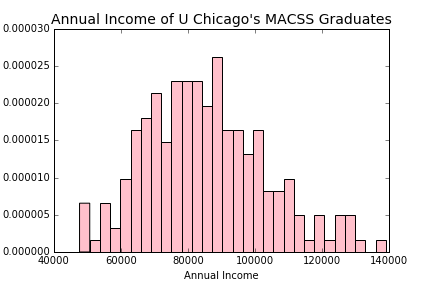
\includegraphics{images/Fig_1a.png}}}
% \end{figure}

